%EQUIVALENT RATIOS \& RATIO TABLES - WORKSHEET 0 (IN-CLASS INSTRUCTION)
\documentclass[12pt, letterpaper, fleqn]{article}

% ----------------------------------------------------------
% PACKAGES
% ----------------------------------------------------------
\usepackage{graphicx}
\usepackage{xcolor}
\usepackage[most]{tcolorbox}
\usepackage{amsmath, amssymb}
\usepackage{fancyhdr}
\usepackage[utf8]{inputenc}
\usepackage[T1]{fontenc}
\usepackage{enumitem}
\usepackage{geometry}
\usepackage{tikz}
\usepackage{needspace}
\usepackage{multicol}

\usetikzlibrary{arrows.meta, calc}

% ----------------------------------------------------------
% PAGE SETUP
% ----------------------------------------------------------
\usepackage{times}
\geometry{letterpaper, top=1.25in, bottom=1.25in, marginpar=0.5in}

% ----------------------------------------------------------
% HEADER / FOOTER
% ----------------------------------------------------------
\newcommand{\logowidth}{3cm}
\setlength{\headheight}{20pt}
\setlength{\footskip}{40pt}

\pagestyle{fancy}
\fancyhf{}
\fancyhead[C]{\small\bfseries Equivalent Ratios \& Ratio Tables}
\fancyfoot[L]{\raisebox{2pt}{
\includegraphics[width=\logowidth]{kss.png}}}
\fancyfoot[C]{\thepage}
\fancyfoot[R]{6.3.0}

\renewcommand{\footrulewidth}{0.2pt}

% ----------------------------------------------------------
% THEME COLOR
% ----------------------------------------------------------
\definecolor{customteal}{HTML}{2fbdb9}

% ----------------------------------------------------------
% HELPER MACROS
% ----------------------------------------------------------
\newcommand{\blank}{\underline{\hspace{2.2cm}}}
\newcommand{\blanklong}{\underline{\hspace{6.5cm}}}
\newcommand{\blankshorter}{\underline{\hspace{1.5cm}}}

% ----------------------------------------------------------
% DOCUMENT
% ----------------------------------------------------------
\begin{document}


\textbf{Name:} \underline{\hspace{5cm}}
\hfill
\textbf{Date:} \underline{\hspace{3cm}}\\

% ==========================================================
% SECTION 1: WHAT ARE EQUIVALENT RATIOS?
% ==========================================================
\begin{tcolorbox}[colback=customteal!20]
    \large\textcolor{black}{\textbf{Equivalent Ratios (Foundation)}}
\end{tcolorbox}

\vspace{3mm}

\noindent
\textbf{Equivalent ratios} are different ratios that show the same relationship. For example:

\vspace{1cm}

\begin{itemize}
    \item $\dfrac{1}{2} = \dfrac{2}{4} = \dfrac{3}{6} = \dfrac{4}{8}$ (all equal to 0.5)
    \item $\dfrac{2}{3} = \dfrac{4}{6} = \dfrac{6}{9} = \dfrac{8}{12}$ (all have the same ratio)
\end{itemize}

\medskip

\vspace{1cm}

\noindent
\textbf{How to Make Equivalent Ratios:} Multiply or divide both the numerator and denominator by the same number.

\vspace{1cm}

\begin{tcolorbox}[colback=white, colframe=black!25, boxrule=0.6pt, arc=4mm, left=6mm, right=6mm, top=5mm, bottom=5mm]

\textbf{Worked Example:} Start with the ratio $\dfrac{2}{5}$

\vspace{0.5cm}

\begin{align*}
\dfrac{2}{5} &= \dfrac{2 \times 2}{5 \times 2} = \dfrac{4}{10} \\ \\
\dfrac{2}{5} &= \dfrac{2 \times 3}{5 \times 3} = \dfrac{6}{15} \\ \\
\dfrac{2}{5} &= \dfrac{2 \times 4}{5 \times 4} = \dfrac{8}{20}
\end{align*}

\vspace{1cm}

\noindent
So $\dfrac{2}{5}$, $\dfrac{4}{10}$, $\dfrac{6}{15}$, and $\dfrac{8}{20}$ are all equivalent ratios.

\end{tcolorbox}

\vspace{4mm}
\newpage
% ==========================================================
% PRACTICE 1: EQUIVALENT RATIOS
% ==========================================================
\begin{tcolorbox}[colback=customteal!20]
\large\textcolor{black}{\textbf{Practice: Find Equivalent Ratios}}
\end{tcolorbox}

\noindent
Multiply both parts of each ratio by the given number.

\vspace{1cm}

\begin{enumerate}[itemsep=3.5cm, leftmargin=0.6cm]
\item $\dfrac{3}{4}$ multiplied by 2: $\dfrac{\phantom{0}}{\phantom{0}}$
\item $\dfrac{5}{6}$ multiplied by 3: $\dfrac{\phantom{0}}{\phantom{0}}$
\item $\dfrac{2}{7}$ multiplied by 4: $\dfrac{\phantom{0}}{\phantom{0}}$
\item $\dfrac{4}{13}$ multiplied by 4: $\dfrac{\phantom{0}}{\phantom{0}}$
\end{enumerate}

\newpage

% ==========================================================
% SECTION 2: RATIO TABLES
% ==========================================================
\begin{tcolorbox}[colback=customteal!20]
\large\textcolor{black}{\textbf{Ratio Tables: Organizing Equivalent Ratios}}
\end{tcolorbox}

\noindent
A \textbf{ratio table} organizes pairs of equivalent ratios in rows and columns. Ratio tables help us see patterns and compare relationships.

\vspace{3mm}

\begin{tcolorbox}[colback=white, colframe=black!25, boxrule=0.6pt, arc=4mm, left=6mm, right=6mm, top=5mm, bottom=5mm]

\textbf{Example: Recipe for Lemonade}

\noindent
The ratio of cups of lemon juice to cups of water is 1:3.

\vspace{1cm}
\begin{center}
\begin{tabular}{|c|c|c|c|c|}
\hline
\textbf{Cups of Lemon Juice} & 1 & 2 & 3 & 4 \\
\hline
\textbf{Cups of Water} & 3 & 6 & 9 & 12 \\
\hline
\end{tabular}
\end{center}
\vspace{1cm}

\noindent
\textbf{Pattern:} The water is always 3 times the lemon juice. Each ratio $\dfrac{1}{3}$, $\dfrac{2}{6}$, $\dfrac{3}{9}$, $\dfrac{4}{12}$ is equivalent.

\end{tcolorbox}

\vspace{1cm}

\begin{tcolorbox}[colback=white, colframe=black!25, boxrule=0.6pt, arc=4mm, left=6mm, right=6mm, top=5mm, bottom=5mm]

\textbf{Example: Scaling Down (Using Division)}

\noindent
Sometimes we need to divide both quantities to find an equivalent ratio or a missing value in our table.

\vspace{1cm}
\begin{center}
\begin{tabular}{|c|c|c|c|}
\hline
\textbf{Miles} & 60 & 30 & 15 \\
\hline
\textbf{Gallons} & 4 & 2 & 1 \\
\hline
\end{tabular}
\end{center}
\vspace{1cm}

\noindent
\textbf{Pattern:} To move left-to-right, we divide both the numerator and denominator by 2 ($\div 2$). Every ratio simplifies down to the unit rate of $\dfrac{15}{1}$.

\end{tcolorbox}

\vspace{4mm}
\newpage

% ==========================================================
% PRACTICE 2: COMPLETE RATIO TABLES
% ==========================================================
\begin{tcolorbox}[colback=customteal!20]
\large\textcolor{black}{\textbf{Practice: Fill in Ratio Tables}}
\end{tcolorbox}

\noindent
Complete each ratio table. Find the pattern and fill in the missing values.

\vspace{3mm}

\noindent
\textbf{1) Ratio 2:5}

\begin{center}
\begin{tabular}{|c|c|c|c|c|}
\hline
\textbf{First} & 2 & 4 & 6 & \phantom{0} \\
\hline
\textbf{Second} & 5 & \phantom{0} & \phantom{0} & 20 \\
\hline
\end{tabular}
\end{center}



\noindent
\textbf{2) Ratio 3:4}

\begin{center}
\begin{tabular}{|c|c|c|c|c|}
\hline
\textbf{First} & 3 & \phantom{0} & 9 & 12 \\
\hline
\textbf{Second} & 4 & 8 & \phantom{0} & \phantom{0} \\
\hline
\end{tabular}
\end{center}



\noindent
\textbf{3) Ratio 5:7}

\begin{center}
\begin{tabular}{|c|c|c|c|c|}
\hline
\textbf{First} & 5 & \phantom{0} & 15 & \phantom{0} \\
\hline
\textbf{Second} & 7 & 14 & \phantom{0} & \phantom{0} \\
\hline
\end{tabular}
\end{center}



\noindent
\textbf{4) Ratio 24:16 (Scaling Down)}

\begin{center}
\begin{tabular}{|c|c|c|c|c|}
\hline
\textbf{First} & 24 & 12 & \phantom{0} & 3 \\
\hline
\textbf{Second} & 16 & \phantom{0} & 4 & \phantom{0} \\
\hline
\end{tabular}
\end{center}

\vspace{4mm}


% ==========================================================
% SECTION 3: FINDING THE SCALE FACTOR
% ==========================================================
\begin{tcolorbox}[colback=customteal!20]
\large\textcolor{black}{\textbf{Scale Factor: The Multiplier in Ratio Tables}}
\end{tcolorbox}

\noindent
The \textbf{scale factor} is the number you multiply by to go from one pair to the next in a ratio table.


\begin{tcolorbox}[colback=white, colframe=black!25, boxrule=0.6pt, arc=4mm, left=6mm, right=6mm, top=5mm, bottom=5mm]

\textbf{Example:}

\begin{center}
\begin{tabular}{|c|c|c|c|}
\hline
& $\times 2$ & $\times 2$ & \\
\hline
\textbf{Miles} & 5 & 10 & 20 \\
\hline
\textbf{Hours} & 2 & 4 & 8 \\
\hline
& $\times 2$ & $\times 2$ & \\
\hline
\end{tabular}
\end{center}

\noindent
The scale factor is 2. Each column is multiplied by 2 to get the next column.

\end{tcolorbox}


% ==========================================================
% THINKING PROBLEM 1
% ==========================================================
\begin{tcolorbox}[colback=white!15, colframe=black, boxrule=1.5pt, arc=4mm, left=6mm, right=6mm, top=5mm, bottom=5mm]

\textbf{Deeper Thinking Problem 1: Comparing Three Store Deals}

\medskip

\noindent
Three different stores sell packs of sports cards:
\begin{itemize}
    \item \textbf{Store A:} 2 packs for \$8
    \item \textbf{Store B:} 3 packs for \$15
    \item \textbf{Store C:} 4 packs for \$12
\end{itemize}

\noindent
\textbf{a)} Complete a mini ratio table for each store to find the cost of 1 pack (the unit rate) and up to 4 packs.

\begin{center}
\textbf{Store A} \ \ \begin{tabular}{|c|c|c|} \hline Packs & 2 & 1 \\ \hline Price & \$8 &   \\ \hline \end{tabular}
\quad \\
\vspace{1cm}
\textbf{Store B} \ \ \begin{tabular}{|c|c|c|} \hline Packs & 3 & 1 \\ \hline Price & \$15 &   \\ \hline \end{tabular}
\quad \\
\vspace{1cm}
\textbf{Store C} \ \ \begin{tabular}{|c|c|c|} \hline Packs & 4 & 1 \\ \hline Price & \$12 &   \\ \hline \end{tabular}
\end{center}

\vspace{2cm}

\noindent
\textbf{b)} Which store offers the best deal (lowest cost per pack)? Explain using the tables.

\vspace{6cm}

\end{tcolorbox}

\newpage

% ==========================================================
% SECTION 4: PLOTTING ON THE COORDINATE PLANE
% ==========================================================
\begin{tcolorbox}[colback=customteal!20]
\large\textcolor{black}{\textbf{Graphing Ratios on the Coordinate Plane}}
\end{tcolorbox}

\noindent
Each pair in a ratio table can be plotted as a point $(x, y)$ on a coordinate plane. The points form a straight line through the origin.

\vspace{3mm}

\begin{tcolorbox}[colback=white, colframe=black!25, boxrule=0.6pt, arc=4mm, left=6mm, right=6mm, top=5mm, bottom=5mm]

\textbf{Example: Ratio 2:3}

\begin{center}
\begin{tabular}{|c|c|c|c|c|}
\hline
\textbf{x (First)} & 2 & 4 & 6 & 8 \\
\hline
\textbf{y (Second)} & 3 & 6 & 9 & 12 \\
\hline
\end{tabular}
\end{center}

\noindent
Points: $(2,3)$, $(4,6)$, $(6,9)$, $(8,12)$

\begin{center}
\begin{tikzpicture}[scale=0.8]
\draw[gray!30] (0,0) grid (10,14);
\draw[->, thick] (-0.5,0) -- (10.5,0) node[right] {x};
\draw[->, thick] (0,-0.5) -- (0,14.5) node[above] {y};
\foreach \x in {2,4,6,8,10} {\draw (\x,-0.1) -- (\x,0.1) node[below=3pt] {\x};}
\foreach \y in {2,4,6,8,10,12} {\draw (-0.1,\y) -- (0.1,\y) node[left=3pt] {\y};}
\plot[only marks, mark=*] coordinates {(2,3) (4,6) (6,9) (8,12)};
\draw (0,0) -- (8,12);
\end{tikzpicture}
\end{center}

\noindent
All points lie on a straight line passing through the origin $(0,0)$.

\end{tcolorbox}

\vspace{4mm}

% ==========================================================
% THINKING PROBLEM 2
% ==========================================================
\begin{tcolorbox}[colback=white!15, colframe=black, boxrule=1.5pt, arc=4mm, left=6mm, right=6mm, top=5mm, bottom=5mm]

\textbf{Deeper Thinking Problem 2: From Graph to Ratio}

\medskip

\noindent
A graph shows the ratio between two quantities. The points are $(1,4)$, $(2,8)$, $(3,12)$, and $(4,16)$.

\noindent
\textbf{a)} What is the ratio of x to y?

\vspace{1.5cm}

\noindent
\textbf{b)} If x = 7, what is y?

\vspace{1.5cm}

\noindent
\textbf{c)} If y = 60, what is x?

\vspace{1.8cm}

\end{tcolorbox}

\vspace{0.5cm}

% ==========================================================
% THINKING PROBLEM 3
% ==========================================================
\begin{tcolorbox}[colback=white!15, colframe=black, boxrule=1.5pt, arc=4mm, left=6mm, right=6mm, top=5mm, bottom=5mm]

\textbf{Deeper Thinking Problem 3: Real-World Application}

\medskip

\noindent
A painter can paint 3 square meters in 2 hours.

\noindent
\textbf{a)} Create a ratio table showing area painted for 2, 4, 6, 8, and 10 hours.

\vspace{2.5cm}

\noindent
\textbf{b)} At this rate, how many square meters can the painter cover in 15 hours?

\vspace{1.5cm}

\noindent
\textbf{c)} How long will it take to paint 45 square meters?

\vspace{1.8cm}

\end{tcolorbox}


\end{document}
\end{document}
